\chapter{相机投影几何的光学约束}
\label{ch:02}

\section{效果}
\label{sec:ch02-effect}

读完本章，你应能：
\begin{enumerate}
  \item 写出含内参矩阵 $K$ 的投影模型，并解释 $f_x,f_y$、主点与像素尺度的光学来源；
  \item 在针孔投影上叠加径向/切向畸变，说明校正顺序与重投影误差的含义；
  \item 陈述景深 $Z_d$ 如何限制「可用于标定与重建的清晰工作距」，以及模糊对特征定位的影响；
  \item 从可观性角度判断：哪些运动与板姿态能把 $K$、畸变与外参 $R,t$ 分开估准，哪些配置会退化。
\end{enumerate}

\section{原理}
\label{sec:ch02-principle}

\subsection{内参 $K$：把光学焦距写成矩阵}

相机坐标系下，点 $\mathbf{X}_c=(X,Y,Z)^\top$（$Z>0$ 在镜头前方的常见约定）先按针孔投影到归一化像平面，再乘内参。像素齐次坐标常写为
\begin{equation}
  s\begin{pmatrix}u\\v\\1\end{pmatrix}
  =
  K\begin{pmatrix}X\\Y\\Z\end{pmatrix},
  \qquad
  K=\begin{pmatrix}f_x & 0 & c_x\\ 0 & f_y & c_y\\ 0&0&1\end{pmatrix},
  \label{eq:ch02-K}
\end{equation}
其中 $s$ 为齐次尺度（齐次因子）。非齐次形式更直观：
\[
  u = f_x\frac{X}{Z}+c_x,\qquad
  v = f_y\frac{Y}{Z}+c_y
  \quad(Z\neq 0).
\]
$f_x,f_y$ 是以像素计的焦距，近似 $f/p_x$、$f/p_y$（$f$ 为毫米焦距，$p_x,p_y$ 为像素间距）；$c_x,c_y$ 为主点，理想上接近光轴与传感器交点的像素坐标。斜歪参数（skew）在现代传感器上常可置零。

光学约束体现在：
\begin{itemize}
  \item $f_x\approx f_y$ 通常接近（方形像素）；显著差异可能来自错误标定或非对称光学；
  \item 主点偏离中心过大时，应怀疑装配、裁切或模型与镜头不匹配；
  \item $K$ 把「毫米光路」接到「像素算法」；$K$ 错则所有三角测量的射线方向错。
\end{itemize}

世界系到相机系：$\mathbf{X}_c=R\mathbf{X}+t$，外参 $R,t$ 描述刚体位姿。多视几何与标定算法见 \citet{HartleyZisserman2004}；平面靶实用流程见 \citet{Zhang2000Calibration}。

\subsection{畸变模型：在归一化平面上改弯}

常用做法：先将像素反投影到归一化坐标 $(x,y)$（未畸变），再施加畸变得到 $(\tilde{x},\tilde{y})$，最后用 $K$ 映回像素——或按实现库的约定顺序严格一致。径向模型示意：
\begin{equation}
  \begin{pmatrix}\tilde{x}\\\tilde{y}\end{pmatrix}
  =
  (1+k_1 r^2+k_2 r^4+\cdots)
  \begin{pmatrix}x\\y\end{pmatrix}
  +\text{切向项},
  \qquad r^2=x^2+y^2.
  \label{eq:ch02-dist}
\end{equation}
$k_1<0$ 常对应桶形倾向，$k_1>0$ 常对应枕形倾向（符号约定因库而异，以文档为准）。切向项刻画偏心等。

\begin{figure}[htbp]
  \centering
  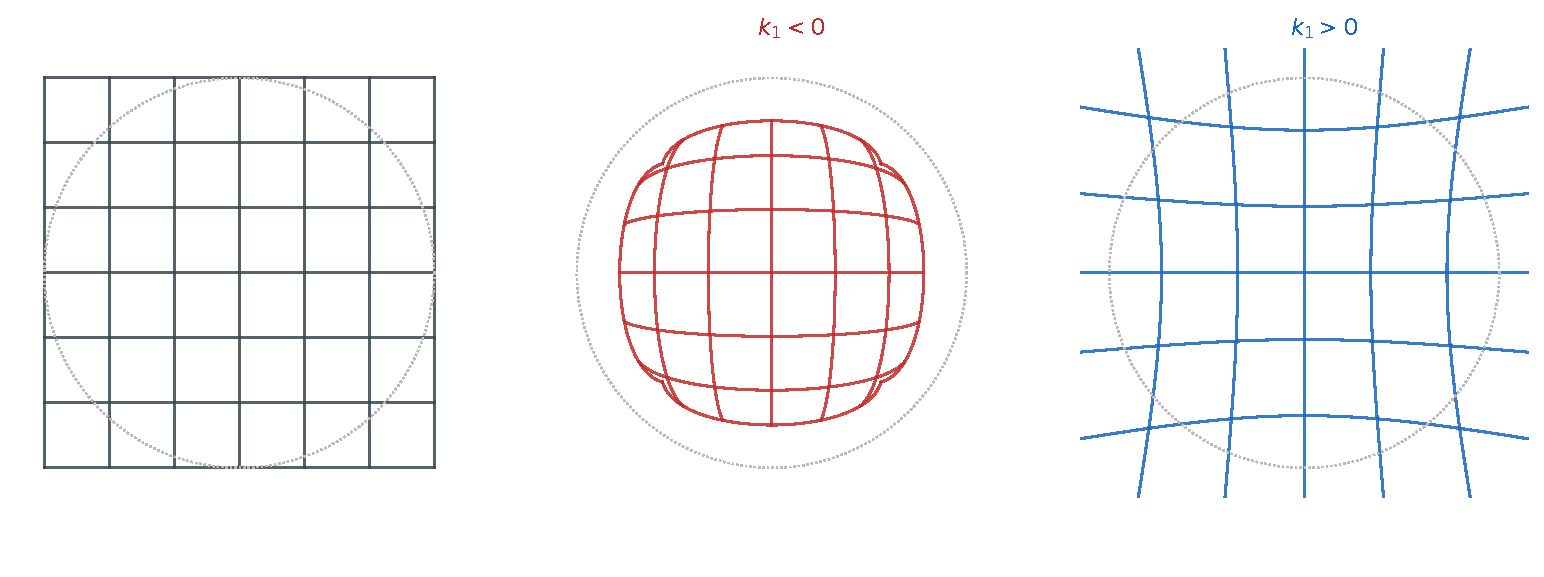
\includegraphics[width=0.95\textwidth]{fig-distortion.pdf}
  \caption{理想网格与桶形/枕形径向畸变概念草图（非精确工程图）。直线在像面上变弯，必须在投影模型中显式建模。}
  \label{fig:ch02-distortion}
\end{figure}

\textbf{重投影误差}：三维点（或标定板上的已知点）经 $R,t$、畸变与 $K$ 预测像素，与检测角点之差。优化标定即减小该类误差。若模型不含畸变，误差会呈径向结构；强行只用 $K$ 会把弯曲「吞进」错误的 $f_x,f_y$ 或主点，留下系统性点云变形。

\subsection{景深、模糊与特征定位}

标定与重建都依赖特征（角点、条纹峰值）的亚像素定位。离焦使 $\PSF$ 展宽，角点响应变钝，定位方差上升；条纹对比度下降等价于频带内 $\SNR$ 变差。因此存在光学约束：
\begin{quote}
有效数据必须落在由 $c_{\max}$ 决定的景深范围（用 $Z_d$ 表征）内；否则估出的 $K$ 或相位是「糊图上的最佳拟合」，泛化到清晰工作距时失效。
\end{quote}
近距大视场时，场曲还会让中心与边缘不能同时最锐（\chapref{ch:01}），标定姿态应覆盖实际扫描的工作距与视场，而非只追求中心一块极锐。

\subsection{标定可观性：什么运动能把参数分开}

平面靶标定 \citep{Zhang2000Calibration} 需要多幅不同姿态。可观性直觉：
\begin{itemize}
  \item \textbf{足够透视变化}：靶面不可总与像面平行且距离不变，否则焦距与深度尺度易纠缠；
  \item \textbf{覆盖视场}：角点应伸到边缘，否则高阶畸变 $k_2,\ldots$ 不可观或过拟合噪声；
  \item \textbf{$Z_d$ 内清晰}：每幅用于标定的图都必须在可接受弥散内；
  \item \textbf{外参与内参}：单目序列中 $R,t$ 每幅不同，$K$ 共享；若错误地让 $K$ 随时间漂，属于过参数化；
  \item \textbf{退化}：所有图像共面运动、视场中央一小块、或几乎纯旋转且无已知尺度时，部分参数方差爆炸。
\end{itemize}

结构光系统还常标定投影仪–相机相对 $R,t$ 与投影仪「内参」。投影仪可类比倒装的相机：其「畸变」与离焦同样存在；条纹相位到射线的映射继承这些误差，并在三角测量中放大（\chapref{ch:07}）。

\subsection{与光学公式的交接}

像素焦距 $f_x$ 随对焦轻微变化（像距 $s'$ 变）；自动对焦扫描头若对焦后仍用旧 $K$，等于系统性改射线方向。浸液、保护窗、温度引起的 $n$ 与机械间隙变化，也会让出厂 $K$ 漂移。工程上：关键工况下定期重标定，并监控重投影误差与点云金标准偏差，而不是假定 $K$ 永恒。


\subsection{从重投影误差到点云误差的数量级直觉}

设角点或相位对应点的像面定位误差为 $\delta u$ 像素，焦距约 $f_x$ 像素，工作距深度 $Z$，基线为 $B$（双目或相机–投影中心距）。三角测量下深度误差常有
\[
  \delta Z \;\sim\; \frac{Z^{2}}{B f_x}\,\delta u
\]
量级关系（系数因几何定义略有不同）。含义：
\begin{itemize}
  \item 同样 $\delta u$，更远或更短基线 → $\delta Z$ 更大；
  \item 离焦或畸变未建模会抬高有效 $\delta u$，并可能引入\textbf{与半径相关的系统} $\delta u$，于是点云出现可重复的弯曲而非仅方差增大；
  \item 标定把 $\delta u$ 的系统部分压下去，比在点云端做各向同性平滑更对症。
\end{itemize}
完整立体限度见 \chapref{ch:07}；本章要求先承认：\textbf{$K$ 与畸变的光学约束通过 $\delta u$ 进入 $\delta Z$}。

\subsection{实现提示（C++/CUDA 视角）}

\begin{itemize}
  \item 畸变校正与投影的顺序必须与标定库一致；在 CUDA 里自写反畸变迭代时，用标定板角点做端到端金标准测试。
  \item 不要把「查找表校正后的图」再送进假定「未校正」的第二套模型。
  \item 对焦电机位置若可读，应记入元数据；任一档位对应一套 $K$ 或一套放大率，禁止混用。
  \item 监控项：每批次标定的重投影 RMS、边缘 vs 中心误差比、以及已知长度量块随 $Z$ 的尺度曲线。
\end{itemize}

\section{限度}
\label{sec:ch02-limits}

\begin{itemize}
  \item 式~\eqref{eq:ch02-K}--\eqref{eq:ch02-dist} 是常用工程模型，不是透镜设计的完整像差展开。
  \item 可观性讨论是定性的；定量协方差依赖角点噪声模型与姿态分布，需用实际标定报告或仿真确认。
  \item 忽略畸变的「也能跑」的 $K$ 在窄视场、弱畸变镜头上可勉强；口内广角常见强畸变，此限度不可忽略。
\end{itemize}

\section{对象}
\label{sec:ch02-object}

\textbf{诊断 1：点云整体「球面感」或边缘外翻。} 先可视化标定板直线是否弯曲、重投影误差是否随半径增大。若是，增强畸变阶数或检查是否用了错误的畸变约定（像素域 vs 归一化域）。对照图~\ref{fig:ch02-distortion} 理解桶/枕方向与 $k_1$ 符号。

\textbf{诊断 2：金标准长度随工作距变化。} 可疑 $f_x,f_y$ 与深度耦合、或对焦后 $K$ 未更新，或窗口玻璃未建模型。在多个 $Z$ 上拍靶，看尺度误差是否单调。

\textbf{诊断 3：标定重投影很小，实地扫描仍差。} 可能标定姿态未覆盖扫描时的 $Z_d$ 与视场（过拟合中心清晰区）；或外参 $R,t$ 在装配后被碰撞改变。用「扫描工况下的再投影 / 再标定」验证，而非只看实验室最优图。

\textbf{诊断 4：左右相机相对位姿不稳。} 双目 $R,t$ 误差直接放大深度；光学上还要保证两路均在 $Z_d$ 内且光照 $\SNR$ 对称，否则匹配偏差被当成几何。


\section*{本章收束}
$K$ 把毫米光路接到像素；畸变在归一化平面改弯；$Z_d$ 约束哪些图能进标定；姿态设计决定可观性。重投影误差与 $\delta Z\sim Z^2\delta u/(B f_x)$ 量级把光学约束接到点云。本编几何与相机部分到此；波动与光度线索从 \chapref{ch:03} 起展开。

\section{习题}
\label{sec:ch02-exercises}

\begin{enumerate}
  \item \textbf{（概念）} 解释 $f_x$ 与薄透镜焦距 $f$（毫米）的关系；像素变小（传感器更密）时，同样光学 $f$ 下 $f_x$ 如何变？
  \item \textbf{（计算）} 设 $f_x=f_y=800$（像素），$c_x=640$，$c_y=360$。相机系点 $(X,Y,Z)=(10,0,200)$（单位任意但一致）。忽略畸变，求像素 $(u,v)$。
  \item \textbf{（计算）} 归一化坐标 $(x,y)=(0.3,0.0)$，$r^2=0.09$，仅径向 $k_1=-0.2$（其余为零）。求畸变后的 $(\tilde{x},\tilde{y})$。相对无畸变，像点更靠近还是更远离中心？
  \item \textbf{（可观性）} 只拍三张几乎平行、距离相同的标定板图像，主要哪类参数难估准？应如何改采集？
  \item \textbf{（重建场景）} 口内头对焦在 $s=25\,\mathrm{mm}$ 后标定；扫描时对焦环被扳到 $s=30\,\mathrm{mm}$ 但未重标。定性预测深度误差类型，并给出处置。
  \item \textbf{（诊断）} 重投影误差中心 $<0.1$~px、四角 $>1$~px，且呈径向。优先加畸变项还是提高角点检测窗口？
  \item \textbf{（综合）} 为何说「景深 $Z_d$」是标定的光学约束而非纯软件选项？举一条违反后的失败模式。
\end{enumerate}

\section{习题讲解}
\label{sec:ch02-solutions}

\begin{enumerate}
  \item $f_x\approx f/p_x$。像素间距 $p_x$ 变小则同样毫米焦距对应更大的 $f_x$（更多像素）。
  \item $u=f_x X/Z+c_x=800\times10/200+640=40+640=680$，$v=c_y=360$。
  \item 因子 $1+k_1 r^2=1-0.2\times0.09=0.982$，故 $(\tilde{x},\tilde{y})=(0.2946,0)$，更靠近中心（桶形倾向示意）。
  \item 焦距与深度尺度、部分畸变可观性差。应改变倾斜角与距离，让透视变化明显，并让角点覆盖边缘。
  \item 像距变化使有效 $f_x,f_y$ 与清晰面改变，射线方向与工作距模型偏离，深度出现与 $Z$ 相关的系统偏差。处置：对焦锁定或对焦后重标；禁止静默扳对焦环。
  \item 优先加/检畸变模型与阶数；单纯加大检测窗口不能消除径向结构系统差。
  \item 标定优化默认特征定位无偏；若图在 $Z_d$ 外，定位偏且糊，得到的 $K$ 不代表清晰工况。失败模式：实验室糊图上误差「还行」，实地清晰扫描边缘点云系统性外翻。
\end{enumerate}
